
\section{Study domain and earthquake data}

Considered events for this study, containing thirty moderate-magnitude earthquakes ($3.5 > M_w > 5.5$) occurred between 1998 and 2014, are spread throughout a simulation domain with a volume projection of \vdomain{180}{135}{62}{km}, which covers the entire Los Angeles metropolitan area and most of the significant geologic structures around. (Fig.~\ref{fig:region}) shows the simlation domain in which we labled the events with sequential letter code from A to Z and AA to AD and Table \ref{tab:events} provides detailed information for those selected events.The unprocessed recorded datafrom SCEC and Strong motion are downloaded for each of the earthquakes to take advantage of the numerous time series available from different data centers. Some of the stations were in common between different networks and some of them were not usable and they needed to be removed. The final number of chosen records for validation for any of the selected earthquake can be found in Table \ref{tab:events}. For almost all of the events there is enough  available stations to make the results of validation acceptable. 

\begin{figure*}
    \centering
    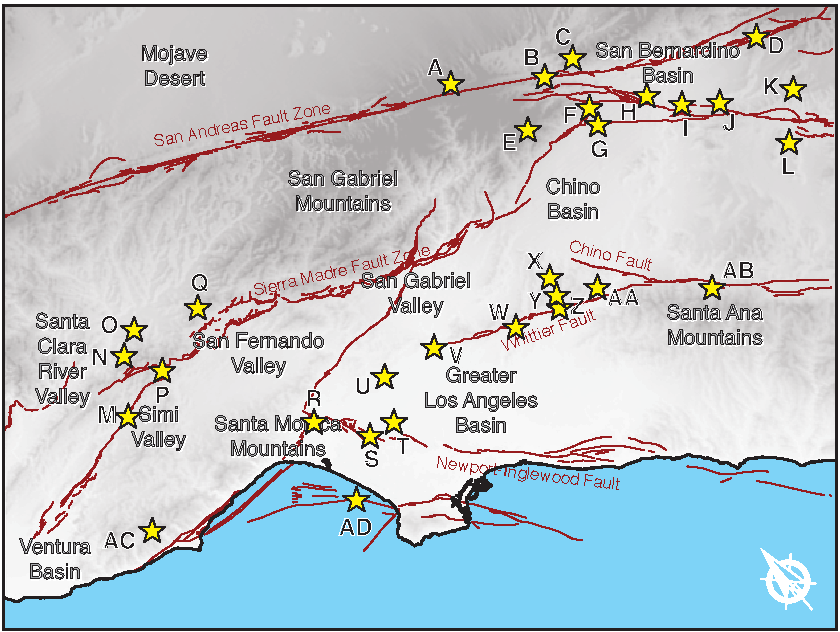
\includegraphics
    	[width=\textwidth]
    	{figures/pdf/figure-01}
    \caption{Region of interest and simulation domain. (a) 3D view of the simulation domain. (b) Geographical location and surface projection of the simulation domain, along with the names of the main cities surrounding the Los Angeles metropolitan are. (c) Major geologic structures including basins, valleys and mountains, along with the main quaternary faults in the region. The color background represents the surface \vsthirty{} values included in the CVM-H+GTL model, with a topography shading effect. The segments $\overline{\mathrm{AB}}$ and $\overline{\mathrm{BC}}$ are used as reference for Fig.~\ref{fig:vslices}.}
    \label{fig:region}
\end{figure*}


\begin{table}
	\centering\small

	\caption{Information for 30 events including their ID \citet{SCEC}, magnitude and final number of stations.}
	\begin{tabular}{|c c c c || c c c c}
	
	\hline

	  	Code								& 
	  	Event ID							& 
	  	\eqmag{w}							&
	  	Num.								&
	  	Code								& 
	  	Event ID							& 
	  	\eqmag{w}							&
	  	Num.								\\
	\hline																																
		A			&	 9064568	&	4.40	&	17&  P&	14312160	&	4.66	&	109	\\ % A 

		B				&	10972299	&	3.79	&	52&	Q&	15237281	&	3.86	&	120\\ % R
		C				&	14494128	&	3.72	&	77&	R&	 9703873	&	4.24	&	130\\ % Z
		D					&	14155260	&	4.88	& 172&	S&	10410337	&	4.70	&	213\\ % V
																					
		E		&	10216101	&	3.60	&	55&	T&	 9716853	&	3.98	&	55\\ % J
																					
		F				&	13692644	&	3.74	&	55&	U&	 9093975	&	3.77	&	25\\ % S
		G				&	14116972	&	4.42	&	83&	V&	14601172	&	4.44	&	180\\ % U
		H			&	10370141	&	4.45	&	159 &	W&	15481673	&	5.10	&	311\\ % L
		I			&	 9140050	&	4.37	&	38&	X&	14383980	&	5.39	&	335\\ % D
		J					&	10541957	& 4.10&	97&	Y&	 9818433	&	4.75	&	67\\ % Q
		K				&	10530013	&	4.28	& 76	& Z&	10399889	&	3.98	&	91\\ % P
		L				&	14239184	&	3.90	&	66&	AA&	 9644101	&	3.64	&	53\\ % W
																					
		M				&	14000376	&	3.59	&	54&	AB&	10275733	&	4.73	&	116\\ % T
		N			&	 9753489	&	3.90	&	52&	AC&	10403777	&	4.42	&	94\\ % H
		O			&	 9096972	&	3.98	&	26&	AD&	14738436	&	3.69	&	93\\ % C
		\hline
																				
	\end{tabular}
	\label{tab:events}
\end{table}



